\documentclass{article}
    \title{\textbf{5. MĚŘICÍ ZESILOVAČE}}
    \author{Tomáš Kysela}
    \date{28/2/2022}

    \addtolength{\topmargin}{-3cm}
    \addtolength{\textheight}{3cm}

\usepackage[czech]{babel}
\usepackage{graphicx}
\usepackage{circuitikz}
\usepackage{amsmath}
\usepackage{subcaption}
\usepackage{pgfplots}
\usepackage{float}
\usepackage[parfill]{parskip}
\usepackage{siunitx}
\sisetup{detect-all}

\makeatletter
\providecommand\add@text{}
\newcommand\tagaddtext[1]{%
    \gdef\add@text{#1\gdef\add@text{}}}%
\renewcommand\tagform@[1]{%
    \maketag@@@{\llap{\add@text\quad}(\ignorespaces#1\unskip\@@italiccorr)}%
}
\makeatother


\begin{document}

\maketitle

\section{Úkol měření}
\begin{enumerate}
	\item Změřte napětí termočlánku předloženým číslicovým voltmetrem pro jednu polohu přepínače termostatu.
	\item S použitím operačního zesilovače OP 07 navrhněte zapojení:
	\begin{enumerate}
		\item invertujícího zesilovače napětí se zesílením -100 a vstupním odporem 1 \si{\kilo\ohm}
		\item neinvertujícího zesilovače napětí se zesílením 100 a vstupním odporem 100 \si{\kilo\ohm}	\end{enumerate}
	\item Invertující zesilovač napětí použijte pro zesílení napětí termočlánku, napětí na výstupu zesilovače změřte stejným číslicovým voltmetrem a pro stejnou  polohu  přepínače termostatu jako v bodě 1. Korigujte chybu metody způsobenou konečným vstupním odporem zesilovače.
	\item Určete rozšířenou nejistotu měření napětí termočlánku (koeficient rozšíření kr = 2) jak pro přímé měření číslicovým voltmetrem, tak pro měření napětí termočlánku  po	zesílení invertujícím zesilovačem napětí.

	Při určení celkové nejistoty typu  B  měření  zesíleného  napětí termočlánku uvažujte i nejistotu způsobenou vstupní napěťovou nesymetrií operačního zesilovače. Nejistoty způsobené vstupními klidovými proudy zesilovače zanedbejte.
	\item Pro polohu přepínače  termostatu použitou při měřeních dle bodů 1 a 3 určete teplotu teplého konce termočlánku (teplotu měřenou termočlánkem), je-li konstanta použitého termočlánku K = 54 \si{\micro\volt\per\degreeCelsius}. Předpokládejte, že teplota srovnávacích (studených) konců termočlánku je 20 °C (teplota laboratoře).
	\item Ověřte, zda je skutečná vstupní napěťová nesymetrie použitého operačního zesilovače menší než maximální (případně typická) hodnota udaná výrobcem.
\end{enumerate}
\textit{Poznámky k měření:}
\begin{enumerate}
	\item Měřte  až  po  dosažení  tepelného  ustálení  obvodu,  které  indikuje  zánik  monotónních  změn údaje číslicového voltmetru (ustálení údaje až na případný vliv šumu).
	\item Tolerance použitých rezistorů a vnitřní odpor termočlánku jsou uvedeny na přípravcích.
	\item Operační zesilovač umožňuje kompenzaci vstupní napěťové nesymetrie a vstupních klidových proudů zesilovače pomocí nastavitelného rezistoru (odporového trimru). V praxi se ale tato kompenzace zpravidla nepoužívá a ani v přípravku není zapojena.
\end{enumerate}

\section{Schéma zapojení}
\begin{figure}[H]
	\centering
	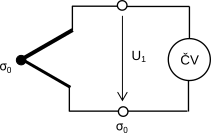
\includegraphics{scheme1}
	\caption{Přímé měření napětí termočlánku číslicovým voltmetrem}
	\label{fig:scheme1}
\end{figure}
\begin{figure}[H]
	\centering
	\begin{subfigure}{0.5\textwidth}
		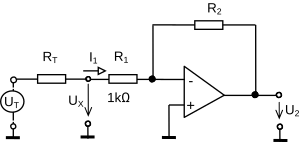
\includegraphics[scale=0.7]{scheme2}
		\caption{Invertující}
		\label{fig:scheme2}
	\end{subfigure}
	\begin{subfigure}{0.45\textwidth}
		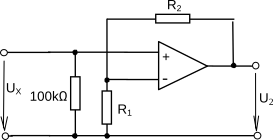
\includegraphics[scale=0.7]{scheme3}
		\caption{Neinvertující}
		\label{fig:scheme3}
	\end{subfigure}
	\caption{zesilovač}
\end{figure}
\begin{table}[h]
	\begin{tabular}{|l||l|l|l|l|l|}
		\hline
		 \textbf{Vlastnost} & \textbf{ICL 7650} & \textbf{741}& \textbf{LT 1097} & \textbf{OP 07}     & \textbf{LM 155} \\ \hline \hline
		napěťový offset  typ./max. (\si{\micro\volt}) & 0.7      & 1500/5000 & 10/60   & 60/150    & 1000   \\ \hline
		jeho teplotní drift (\si{\micro\volt\per\degreeCelsius})     & 0.02     & 10        & 0.3     & 0.5       & 5      \\ \hline
		jeho teplotní drift (\si{\micro\volt\per\degreeCelsius})     & 5        & 50000     & 350     & 1800/7000 & 50     \\ \hline
		CMRR (\si{\decibel})                       & 120      & 90        & 130     & 110       & 100    \\ \hline
		rychlost přeběhu (\si{\volt\per\second})         & 2.5      & 0.5       & 0.2     & 0.3       & 5      \\ \hline
	\end{tabular}
\end{table}
\section{Soupis použitých přístrojů}



\section{Teoretický základ}
\subsection{Kontrola vstupní napěťové nesymetrie}
Vstupní napěťovou nesymetrii invertujícího zesilovače zjistíme změřením výstupního napětí tohoto zesilovače při zkratovaném vstupu a vydělením tohoto napětí zesílením zesilovače pro napěťovou nesymetrii, které je v našem případě rovno 101 (pro odpory $R_1 = 1 \si{\kilo\ohm}$ a $R_2 = 100 \si{\kilo\ohm}$ a při uvážení skutečnosti, že napětí napěťové nesymetrie je zesilováno neinvertujícím zesilovačem)

\subsection{Určení nejistot}
Při měření výstupního napětí $U_1$, které je úměrné rozdílu teplot $\vartheta_1 - \vartheta_0$ ohřívaného spoje a laboratoře, číslicovým voltmetrem, určíme jeho std. nejistotu jako:
\begin{equation}
    u_{U1}=\frac{	| \frac{\sigma_1}{100}U_1 | + | \frac{\sigma_2}{100}U_R | }{\sqrt{3}}
\end{equation}
kde $\sigma_1$ je chyba v \% měřené hodnoty a $\sigma_2$ je chyba v \% rozsahu$U_R$. Relativní standardní nejistota měření napětí číslicovým voltmetrem je
\begin{equation}
    u_{U1,r} = \frac{u_{U1}}{U_1} \cdot 100\%
\end{equation}
Pro $U_2$ platí obdobné vztahy. V této úloze měříme napětí termočlánku, které je tak malé, že údaj voltmetru je při přímém měření na začátku měřicího rozsahu. Pokud budeme měřit napětí až po zesílení, ale na stejném rozsahu voltmetru se sice drobně zvýší první ze složek nejistoty, nicméně druhá složka se sníží tolikrát, kolikrát se napětí zvýší. Proto je výhodné napětí před měřením zesílit. Tato výhoda se ovšem výrazně neprojeví, pokud je po zesílení napětí nutno přepnout rozsah voltmetru a pokud je pro zesílení použit nekvalitní opera ční zesilovač s velkou vstupní napěťovou nesymetrií.

Hodnota odporu termočlánku $R_T$ je uvedena na přípravku, řádově jednotky ohmů. Úbytek napětí na tomto odporu vyvolaný vstupním proudem voltmetru způsobí, že měřené napětí je menší než napětí na termočlánku, jelikož měříme napětí $U_T$ tvořeného $R_T$ a $R_V$. Tuto systematickou chybu je možno korigovat. Pro napětí termočlánku $U_T$ a měřené napětí $U_X$ platí vztah:
\begin{equation}
    U_X = \frac{R_V}{R_V+R_T}U_T
\end{equation}
Při měření napětí až po zesílení musíme při výpočtu celkové nejistoty měření uvážit složky nejistoty typu B působené tolerancemi odporů zpětnovazební smyčky zesilovače, vstupními proudy a vstupní napěťovou nesymetrií zesilovače a výše zmíněnou metodickou chybu (způsobenou zde konečným vstupním odporem zesilovače).

\subsubsection{Invertující OZ}
Pro ideální invertující OZ (obr. 2a) platí:
\begin{equation}
    U_X=-\frac{R_1}{R_2}U_2
\end{equation}
kde $U_2$ je výstupní napětí zesilovače a $U_X$ je měřené napětí termočlánku. Odpor $R_1$ určuje vstupní odpor zesilovače a volí se tedy podle zadání $1 \si{\kilo\ohm}$. Odpor $R_2$ bude tedy $100 \si{\kilo\ohm}$, abychom dosáhli požadovaného zesílení -100.

Naměřenou hodnotu napětí termočlánku ovlivní také chyba metody, způsobená zatížením termočlánku vstupním odporem měřícího zařízení. Takto vzniklou chybu můžeme odstranit vynásobením $U_X$ korekčním činitelem:
\begin{equation}
    U_T = U_X K_F = U_X \frac{R_1+R_T}{R_1} = U_X (1+\frac{R_T}{R_1})
\end{equation}
Složka standardní nejistoty typu B měření napětí $U_X$ způsobená tolerancemi odporu rezistorů a chybou číslicového voltmetru je pro případ ideálního operačního zesilovače dána vztahem
\begin{equation}
    u_{Ux(id)}=\sqrt{(\frac{\partial U_X}{\partial R_1}u_{R1})^2 + (\frac{\partial U_X}{\partial R_2}u_{R2})^2 + (\frac{\partial U_X}{\partial U_2}u_{U2})^2}
\end{equation}
Kromě této složky se na nejistotě typu B podílí také složka působená nedokonalostmi reálného operačního zesilovače (nenulovými vstupními klidovými proudy $I_{1P}$ a $I{1N}$ a nenulovou vstupní napěťovou nesymetrií $U_{D0}$):
\begin{equation}
    U_X=-\frac{R_1}{R_2}U_2 \mp I_{1N}R_1\pm U_{D0}(1+\frac{R_1}{R_2})
\end{equation}
Složka standardní nejistoty napětí $U_{X}$ odpovídající vstupní napěťové nesymetrii $U_{D0}$ je
tedy
\begin{equation}
    u_{OZ(U_{D0})} = \frac{U_{D0}}{\sqrt{3}}(1+\frac{R_1}{R_2})
\end{equation}
Celková nejistota měření napětí $U_{X}$ při použití reálného zesilovače je při zanedbání vlivu
vstupního klidového proudu $I_{1N}$ tedy
\begin{equation}
    u_{U_X(OA)}=\sqrt{u_{U_X(id)}^2+u_{OA(U_{D0})}^2}
\end{equation}

\subsubsection{Neinvertující OZ}
Při měření se zesilovačem v neinvertujícím zapojení (obr. 2b) platí
\begin{equation}
    U_X=\frac{R_1}{R_2+R_1}U_2
\end{equation}
Standardní nejistotu měřeného napětí lze tedy určit (podle zákona šíření nejistot) jako
\begin{equation}
    u_{Ux(id)}=\sqrt{(\frac{\partial U_X}{\partial R_1}u_{R1})^2 + (\frac{\partial U_X}{\partial R_2}u_{R2})^2 + (\frac{\partial U_X}{\partial U_2}u_{U2})^2}
\end{equation}
U reálného OZ pak dostaneme vztah
\begin{equation}
    U_X=\frac{R_1}{R_1+R_2}U_2 \mp I_{1N}R_2\frac{R_1}{R_1+R_2}\pm U_{D0}
\end{equation}
Výsledná std. nejistota typu B je poté dána vztahem
\begin{equation}
    u_{U_X(OA)}=\sqrt{u_{U_X(id)}^2+u_{OA(I_{1N})}^2+u_{OA(U_{D0})}^2}
\end{equation}
\subsection{Určení teploty}
Výpočet teploty teplého konce termočlánku ze změřeného napětí termočlánku se provede podle přibližného vztahu
\begin{equation}
    \vartheta_1=\frac{U_1}{K}+\vartheta_0
\end{equation}
kde $K = 54 \cdot 10^{-6} \si{\volt\per\degreeCelsius}$. Teplotu okolí předpokládáme $\vartheta_0 = 20 \si{\degreeCelsius}$.
\end{document}